\subsection{Potential Energy Function: The Force Field}\label{subsec:FF}

A bio-molecular force field generally consists of potential energy terms representing covalent interactions between atoms (such as bond-stretching, bond-angle bending, improper and proper dihedral-angle torsion), and non-bonded interactions between atoms in different molecules and between atoms in a molecule that are separated by more than two or three covalent bonds \cite{van2006biomolecular}. Consider a system that contains $N$ particles that are treated explicitly in the model. Often, these particles are atoms, but also groups of atoms can be treated as a single particle, such as hydrocarbons  like $CH , CH_{2} , CH_{4}$ groups. In classical simulations, the system is fully defined by the positions $\textbf{``q"}$, and the conjugate momenta, $\textbf{``p"}$, of the individual particles, where $r$ and $p$ represent 3-N dimensional vectors. In this work, we will use $q_{i}$ and $p_{i}$ for the three-dimensional vectors describing the position and momentum of the particle $``i"$. The potential energy function that determine the system, the \textbf{Hamiltonian}, is written as:
\begin{equation}
    H(p,q)= K(p)+V(q)
    \label{eq:hamiltonian}
\end{equation}
where $K(p)$ is the kinetic energy which can be
\begin{equation}
    K(p,m)=\sum_{i=1}^{N} \frac{p_{i}^{2}}{2m_{i}} = \sum_{i=1}^{N} \frac{1}{2}m_{i}v_{i}^{2}
\end{equation}
$V(r)$ in equation \ref{eq:hamiltonian} is the potential energy, describing the interaction between the particles in the system and possibly external influences on the system. It's a function of the particle position $\textbf{``q"}$. The functional form and parameters describing $V(r)$ is called \textbf{force field}. There are several well-known force fields for biomolecular simulation described in the literature, such as AMBER \cite{amber}, CHARMM \cite{charmm}, ECEPP/3 \cite{ECEPP/3}, and GROMOS \cite{van2005gromacs}\cite{gromos1}, and it takes different forms depending on the description of the system, and is usually a sum of multiple potential energy terms which describe different contributions corresponding to physical (or special) interactions. The potential energy is usually written as a sum over different contributions, separated in physical interactions and any special (unphysical, such as distance restraints between atoms and positional restrains) interaction one might want to apply to the system
\begin{equation}
    V(q)=V^{phys}(q) + V^{special}(q)
    \label{eq:v_general}
\end{equation}
The first term of Equation \ref{eq:v_general} is the mathematical description of the sum of various terms describing the bonded (bon) and nonbonded (nonb) interactions between particles. Bonded potential energy can be divided further to account for bonds, bond angles, harmonic (improper) dihedral angles and torsional or proper dihedral angles (Equation \ref{eq:bond_inter}), and not bonded interaction are are the sum of electrostatic (Coulomb) and van der Waals (Lennard-Jones potential) interactions between pairs of atoms (Equation \ref{eq:nonb_inter}).
\begin{equation}
    V^{bon}(q)= V^{bond}(q)+ V^{angle}(q)+ V^{imp}(q)+ V^{tor}(q)
    \label{eq:bond_inter}
\end{equation}
\begin{equation}
     V^{nonb}(q)=  V^{vdw}(q)+ V^{elec}(q)
     \label{eq:nonb_inter}
\end{equation}

\subsubsection{Force-Field Bonded Interactions}

In the followin sections, $V^{bon}$ terms are explain according to the GROMOS force field which is use in this work.

\subsubsection*{Bond stretching force-field term}
The potential energy term associated with bond-stretching interactions is the term $V^{bond}(q)$ in Equation \ref{eq:bond_inter} and it's the function describing the potential energy associated with the stretching of a single bond and has the form of an harmonic oscillator given by:
\begin{equation}
    V^{bond}(q) = \sum_{n=1}^{N}\frac{1}{2}k_{b}{(b_{n}-b_{n}^{0})}^2
    \label{eq:pot_bond}
\end{equation}
where the quantities $k_{b}$ and $b_{n}$ represent force-field parameters, force constant and reference length, respectively, characteristic for the specific bond n, and $N$ the total number of covalent bonds. 


\subsubsection*{Bond-angle bending force-field term}
The potential energy term associated with bond angle bending interactions is the term $V^{angle}(q)$ in Equation \ref{eq:bond_inter}. Each definable covalent bond angle associated with one and only one bending term in the GROMOS force and this term represent the function describing the potential energy associated with the bending of a single bond angle. It's given by: 
\begin{equation}
    V^{angle}(q)=\sum_{n=1}^{N}\frac{1}{2}k_{\theta }{(\theta_{n}-\theta _{n}^{0})}^2
    \label{eq:angle_bond}
\end{equation}
where $k_{\theta }$ and $\theta _{n}$ represent force-field parameters, force constant and reference bond angle, respectively, characteristic for the specific bond angle n. 

\subsubsection*{Improper dihedral-angle bending force-field term}

The potential energy term associated with improper dihedral-angle bending interactions, typically controlling out-of-plane or out-of-tetrahedron distortions, is the term $V^{imp}(q)$. Improper dihedral angles are used to select the correct geometry or chirality of atoms. The mathemtaical expression is given by:
\begin{equation}
    V^{imp}(q)=\sum_{n=1}^{N}\frac{1}{2}k_{\xi}{(\xi_{n}-\xi_{n}^{0})}^2
    \label{eq:improper_bond}
\end{equation}
where $k_{\xi}$ and represent the force-field force constant for each $\xi_{n}$ represents the value of improper dihedral angle n in the given system configuration, \textit{i.e.}, the dihedral angle formed by the four atoms. 

\subsubsection*{Proper dihedral-angle torsion force-field term}
The potential energy term associated with torsional dihedral-angle bending interactions, is typically controlling, together with non-bonded interactions, the rotational barriers around covalent bonds. $V^{tor}(q)$ is the function describing the potential energy contribution of the term to the torsion of the corresponding proper dihedral angle.
\begin{equation}
     V^{tor}(q)=\sum_{n=1}^{N}k_{\phi}(1+cos(n\phi-\delta)
     \label{eq:torcional_bond}
\end{equation}
where $k_{\phi}$ is the force constant define by the force field, $\delta$ the phase shift (which corresponds to the minimum energy angle), n is the multiplicity (number of minima of the potential energy as it rotates a full 360 degrees), and $\phi$ is the dihedral angle.

In Figure \ref{fig:bonded_inter} are represented each of the potential energy terms described above and the main interaction that the potential describes.

\begin{figure}[ht]

    \centering
    \begin{subfigure}[t]{0.25\textwidth}
    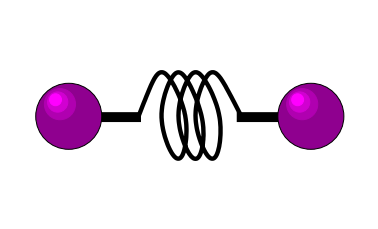
\includegraphics[width=\textwidth]{Figures/Chapter2/bond.png}
    \caption{Bond stretching force-field representation}
    \label{fig:bond}
    \end{subfigure}
    \hspace{1cm}
    \begin{subfigure}[t]{0.25\textwidth}
    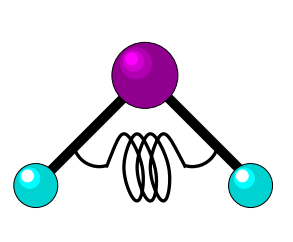
\includegraphics[width=\textwidth]{Figures/Chapter2/angle.png}
    \caption{Bond-angle bending force-field representation}
    \label{fig:angle}
    \end{subfigure}
    
    \begin{subfigure}[t]{0.25\textwidth}
    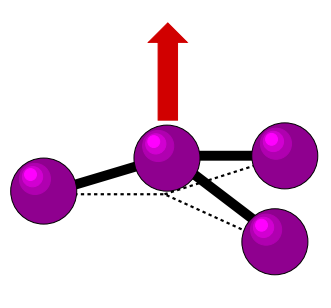
\includegraphics[width=\textwidth]{Figures/Chapter2/impropial.png}
    \caption{Improper dihedral-angle bending force-field representation}
    \label{fig:impropial}
    \end{subfigure}
    \hspace{1cm}
    \begin{subfigure}[t]{0.25\textwidth}
    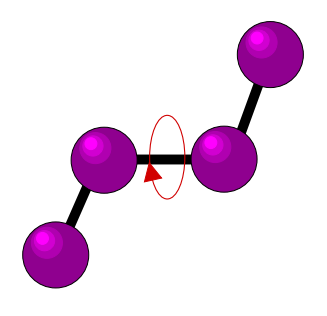
\includegraphics[width=\textwidth]{Figures/Chapter2/torsional.png}
    \caption{Proper dihedral-angle torsion force-field representation }
    \label{fig:torsional}
    \end{subfigure}
    
    
    \caption{Illustration of the various terms included in an empirical potential energy function. Figure adapted from C. Chipot \cite{chipot2010numerical}}
    \label{fig:bonded_inter}
    
\end{figure}

As it is presented in Section \ref{subsec:molecular_structure}, the main objective of this work is to evaluate the non-bonded interactions between the solvent and the solute, particularly the van der Waals interaction. To formulate a complete description of the non-bonded interaction described in Equation \ref{eq:v_general}, the following section is focus on describe the detail mathematical formulation of the terms involved in Equation \ref{eq:nonb_inter}.  

\subsubsection{Force-Field Non-bonded Interactions}

In addition to the bonded interactions between atoms described above, force fields also contain non-bonded interactions. Non-bonded interactions act between atoms in the same molecule and those in other molecules. Force fields usually divide non-bonded interactions into two: Electrostatic interactions and van der Waals interactions.

\subsubsection*{Electrostatic Interactions}
Electrostatic or Coulomb potential describes the interactions potential between pairs of partial charges and it's given by de Coluomb's law.
\begin{equation}
    V^{elec}(q)=\frac{1}{4\pi\epsilon_{0}\epsilon_{1}}\sum_{i=1}^{N-1}\sum_{j=i+1}^{N}\frac{q_{i}q_{j}}{r_{ij}}
    \label{eq:electrostatic}
\end{equation}
where $\epsilon_{0}$ is the dielectric permittivity of vacuum, $\epsilon_{1}$ the relative permittivity of the medium, $q_{i}$ and $q_{j}$ are the charges of atoms $i$ and $j$ involved in the interaction, and $r_{ij}$ the distance between the atoms. 

\subsubsection*{Van der Waals Interactions. The Lenard-Jones Potential}\label{subsubsec:LJ}
The van der Waals force is a weak, short-range force that arises from temporal fluctuations of the charge distribution. This force can attract ideal gas atoms together. Ideal gas atoms are electrically neutral (Figure \ref{fig:vdw_1}) so there is no Coulomb attraction between them. The average dipole moment of an ideal gas atom is zero but the charge fluctuates around its average position and can temporarily create a dipole moment (Figure \ref{fig:vdw_2}). This dipole moment induces a response in the neighboring atom such that there is a net attractive force between the atoms (Figure \ref{fig:vdw_3}). The average over the attractive forces caused by the charge fluctuations is the van der Walls force.

\begin{figure}
    \centering
    \begin{subfigure}[t]{0.25\textwidth}
    
\includegraphics[width=\textwidth]{Figures/Chapter2/vdw1.png}
    \caption{Graphic representation of two neutral atoms.}
    \label{fig:vdw_1}
    \end{subfigure}
    \hspace{0.5cm}
    \begin{subfigure}[t]{0.25\textwidth}
    
\includegraphics[width=\textwidth]{Figures/Chapter2/vdw2.png}
    \caption{A charge fluctuation creates a dipole.}
    \label{fig:vdw_2}
    \end{subfigure}
    \hspace{0.5cm}
    \begin{subfigure}[t]{0.25\textwidth}
    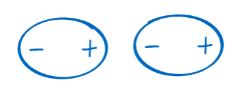
\includegraphics[width=\textwidth]{Figures/Chapter2/vdw3.png}
    \caption{The dipole induces a dipole on the other atom.}
    \label{fig:vdw_3}
    \end{subfigure}
   
    \caption{Illustration of the sequence of events that generates the Van der Waals forces.}
    \label{fig:van_der_waals}
\end{figure}

The Van der Waal bond potential is often approximated by a Lennard-Jones model which consist of two components: a steep repulsive term, $(\sigma/r_{ij})^{12}$ and a smoother attractive term, $(\sigma/r_{ij})^{6}$ as it is shown in Figure \ref{eq:LJ_pot}, which respectively denote repulsive and attractive force. The mathematical description of this potential is given by: 
\begin{equation}
    V^{vdw}(r_{ij})=4\epsilon\left [\left ( \frac{\sigma}{r_{ij}} \right )^{12}-\left (\frac{\sigma}{r_{ij}} \right )^{6} \right ] 
    \label{eq:LJ_pot} 
\end{equation}
where $\epsilon$ is the well depth and a measure of how strongly the two particles attract each other, and $\sigma$ is the distance at which the inter-molecular potential between the two particles is zero as it's shown in Figure \ref{fig:LJ_1}. It gives a measurement of how close two non-bonding particles can get and $r_{ij}$ is the distance of separation between both particles measured from the center of one particle to the center of the other particle.
\begin{figure}[h]
    \centering
    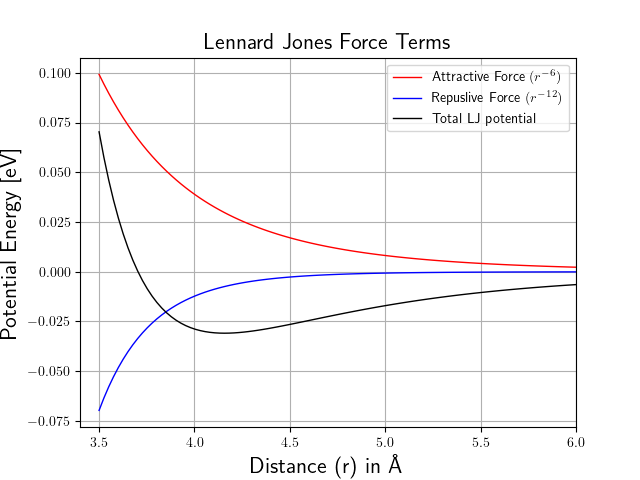
\includegraphics[scale=0.6]{Figures/Chapter2/LJ_1.png}
    \caption{Graphic representation of the attractive and repulsive terms of the Lenard Jones Potential}
    \label{fig:LJ_1}
\end{figure}

Like the bonding potential energy, the stability of an arrangement of atoms is a function of the Lennard-Jones separation distance. As the separation distance decreases below equilibrium, the potential energy becomes increasingly positive (indicating a repulsive force). Such a large potential energy is energetically unfavorable, as it indicates an overlapping of atomic orbitals. However, at long separation distances, the potential energy is negative and approaches zero as the separation distance increases to infinity (indicating an attractive force). This indicates that at long-range distances, the pair of atoms or molecules experiences a small stabilizing force. Lastly, as the separation between the two particles reaches a distance slightly greater than $\sigma$, the potential energy reaches a minimum value (indicating zero force) which is represented by $r_{min}$ in Figure \ref{fig:LJ_parameters}. At this point, the pair of particles is most stable and will remain in that orientation until an external force is exerted upon it. 
\begin{figure}[h]
    \centering
    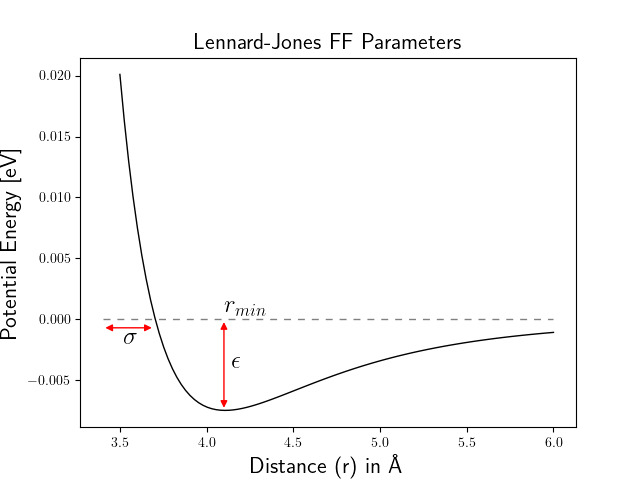
\includegraphics[scale=0.6]{Figures/Chapter2/LJ_2.png}
    \caption{The Lennard-Jones Potential curve, calculated for $\epsilon$ = 0.0103 and $\sigma$ = 3.8.}
    \label{fig:LJ_parameters}
\end{figure}
\begin{equation}
    r_{min}(ij)= 2^{1/6}\sigma
    \label{eq:r_min}
\end{equation}

There are several different ways to formulate the Lennard-Jones potential besides Equation \ref{eq:LJ_pot}, the most common form in the literature is the \textbf{AB potential} and is frequently used in implementations of simulation software as it is computationally favorable. The Lennard-Jones potential can be written as:
\begin{equation}
    V^{LJ}(r_{ij})=\frac{A}{r_{ij}^{12}}-\frac{B}{r_{ij}^{6}} 
    \label{eq:AB_LJ_pot}
\end{equation}
where 
\begin{align*}
    A&=4\epsilon\sigma^{12} & B&=4\epsilon\sigma^{6} & \sigma&=\sqrt[6]{\frac{A}{B}} & \epsilon&=\frac{B^{2}}{4A}
\end{align*}
In GROMOS, the van der Waals (vdw) interaction term $V^{vdw}$ in Equation \ref{eq:nonb_inter} is represented by a Lennard-Jones function, and the term is partitioned as a sum of two contributions. It's given by:
\begin{equation}
    V^{vdw}(r_{ij})=\sum_{i=1}^{N-1}\sum_{j=i+1}^{N} \left [  \frac{C_{12}(i,j)}{r_{ij}^6}-C_{6}(i,j) \right ]\cdot \frac{1}{r_{ij}^6}
    \label{eq:gromos_LJ}
\end{equation}
and every $C_{12}(i,j)$, $C_{6}(i,j)$ is easily extracted from the force-field parameters file in the GROMOS software. More about how GROMOS work is discussed in Section \ref{subsec:about_}. Finally, the total potential energy involved in the therm $V(q)$ from Equation \ref{eq:hamiltonian} it's determined by the sum of every potential energy described in this section, for the pair of atoms $(i,j)$.


